\documentclass{article}
\usepackage{longtable}
\usepackage{makecell}
\usepackage{float}
\usepackage{graphicx}
\usepackage{bm}
\usepackage{placeins}
\usepackage{booktabs}
\usepackage{gensymb}
\usepackage{amssymb}
\usepackage{indentfirst}
\usepackage{threeparttable} 
\usepackage{multirow}
\usepackage{aligned-overset}
\usepackage[slantfont,boldfont]{xeCJK}
\usepackage{fontspec}
\renewcommand{\arraystretch}{1.5}
\usepackage[paperwidth=20cm,paperheight=33.3cm]{geometry}
\setCJKmainfont{SimSun}
\setmainfont{SimSun}
\setsansfont{SimSun}

\title{弦振动实验报告}
\author{2411545 邱凯锐}
\date{2025.5.12}

\begin{document}
\maketitle
\section{实验目的}
1. 掌握在弦线上形成稳定驻波的方法,观察驻波的形成过程;

2. 用两种不同的方法测定电动音叉的频率;

3. 用最小二乘原理拟合直线,验证波长与弦线张力的关系; 
\section{引言}
一切机械波,在有限大小的物体中进行传播时会形成各式各样的驻波。驻波是常见的一种波的迭加现象,它广泛存在于自然界中,如管、弦、膜、板的振动都可形成驻波。驻波理论在声学、光学及无线电中,都有着重要的应用,如用来测定波长、波速或确定波动频率等。

一般的驻波发生在三维空间,较为复杂。为了便于掌握其基本特征,本实验研究最简单的一维空间的情况,即通过研究一根弦线的振动情况,以观察驻波的形成过程,获得稳定驻波的条件和调节方法,以及在弦的线密度基本不变的情况下,研究波长随弦线张力的变化关系,且由此还可以求出电动音叉的固有频率。 
\section{实验原理}
设有两列波在横轴上传播,如Figure 1所示,其振幅、频率及振动方向均相同,但传播相反,向右的以实线表之,向左的以虚线表之。当\(t = 0\)时,两波互相重叠,其合成波如Figure 1 (a)中粗实线所示,此时各点位移最大。\(t = T/4\)时,两列波分别在其传播方向上向右和向左移动\(1/4\)波长的距离,合成波上各点的位移为零,如Figure 1 (b)。\(t = T/2\)时两相干波又相互重叠,各点位移最大,但位移方向却与\(t = 0\)时相反[如Figure 1 (c)]。由此可知,上述二相干波叠加后,使横轴上某些点的振幅为零,称为波节,以“0”表示;而有些点的振幅则有最大值,且等于单个波振幅的2倍,称为波腹,以“+”表示。从外形看合成波波腹和波节的位置不随时间改变,波形不向前传播,故这种波称为驻波。如Figure 2所示。在驻波上,两个相邻的波节或波腹间的距离为半个波长,即:\(\lambda/2\)。因此,可以很方便地测出波长,这就是驻波的重要用途之一。

\begin{figure}[ht]
    \centering
    \begin{minipage}{0.45\textwidth} % 调整宽度为总宽度的45%
        \centering
        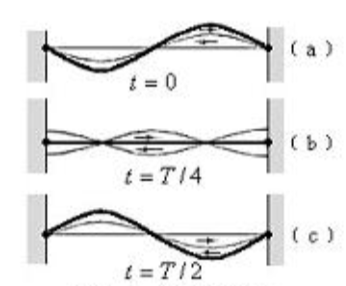
\includegraphics[width=5cm]{1.png} % 替换为你的图片路径
        \caption{驻波的形成}
    \end{minipage}\hfill
    \begin{minipage}{0.45\textwidth}
        \centering
        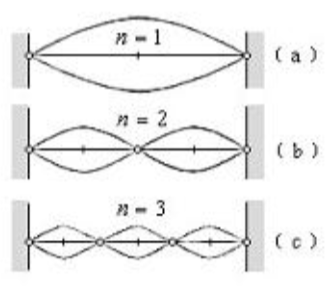
\includegraphics[width=5cm]{2.png} % 替换为你的图片路径
        \caption{弦线上的驻波}
    \end{minipage}
\end{figure}

驻波的形成,通常是在入射波与反射波相互叠加的情况下发生的。如果把弦线的一端$A$固定在音叉上,另一端通过滑轮系上砝码$m$,使弦线中产生一定张力$T$;弦线因穿过支架$B$上的小孔而使该点不能振动。当音叉按自己的固有频率$f$振动时,入射波由$A$向$B$方向传播,并在$B$点发生反射,形成由$B$向$A$的反射波,入射波和反射波的频率、振幅和振动方向都相同,只是传播方向相反,满足驻波形成的条件。若$A$、$B$间的距离即弦长$l$恰为半波长的整数倍,即:

\begin{equation}
    l = n\cdot\frac{\lambda}{2}
\end{equation}

则可在\(A\)、\(B\)之间形成稳定的驻波,如图Figure 2所示。这是因为,当波在两种介质的分界面上发生反射时,若波从波阻较大的介质中反射回来,则反射处形成波节,而与音叉连接的\(A\)端振幅甚小,亦可视为“波节”。

为在弦线上获得稳定的驻波,可采取两种方法:一种是固定弦长\(l\),改变\(T\),另一种是固定张力\(T\),改变\(l\)。本实验即是通过改变支架\(B\)的位置来获得稳定驻波的。弦线上形成稳定驻波的特点是:波节的位置不变,波腹最大且稳定。

根据弹性理论,当横波沿弦线传播时,在维持弦线张力\(T\)不变的情况下,波的传播速度\(v\)与张力及弦线的线密度\(\rho\)之间有如下关系:
\begin{equation}
v = \sqrt{T / \rho}
\end{equation}
而波长\(\lambda\)、频率\(f\)及波速之间的关系为:
\begin{equation}
v = \lambda f
\end{equation}
因此,
\begin{equation}
\lambda = \frac{1}{f}\sqrt{T / \rho}
\end{equation}

式(4)表示:当弦线的线密度不变时,波长与弦线的张力\(T\)的平方根成正比。将式(1)代入式(4),可得:

\begin{equation}
f = \frac{n}{2l}\sqrt{T / \rho}
\end{equation}

式(5)表明,若知道\(\rho\)及\(T\),只要测出稳定驻波形成后\(n\)个半波长之间的距离\(l\),即可求出音叉的固有频率\(f\)。本实验中为了便于测量和计算,可以只测两个半波长(\(n = 2\))间的距离[如Figure 2(b)],即直接测定波长\(\lambda\)。于是,频率可由下式计算:

\begin{equation}
f = \frac{1}{\lambda}\sqrt{T / \rho}
\end{equation}

\section{实验仪器及调节}
电动音叉、滑轮、弦线、砝码组、支架及米尺等。

调节音叉起振时,应轻缓拧动螺丝K,当与弹片接触并产生蓝色火花时即已起振。继续拧动螺丝K,音叉振动加强,至强度适中(以电磁铁不撞击音叉臂为宜)即可停止拧动K。为防止火花间隙改变而使振动强度发生改变或停振,应旋紧调节螺丝上的锁紧螺母。

起振后,在一定张力\(T = mg\) 作用下,移动支架B,适当改变弦长,即可形成稳定驻波。稳定驻波形成后,将支架C移至某波节下面,即可由米尺测定弦长。若取\(n = 2\),则弦长即波长\(\lambda\)。

\section{实验内容}
\subsection{测量弦线的线密度$\rho$}
测量弦线的总长度$L$和总质量$M$,计算得到弦线的线密度$\rho=\frac{M}{L}$。
\subsection{固定张力$T$,改变$l$}
在砝码质量为100g(包括砝码托)的情况下,移动支架B使A、B间形成尽可能多的稳定驻波数,用米尺测出B、C间一个波长的距离4次(每次测量应重新调节)。然后根据给定弦线密度求音叉的固有频率。 
\subsection{固定弦长$l$,改变$T$}
在不同张力 \(T_i = 50, 70, 100, 130, 160, 200 (9.8\times10^{-3} \mathrm{N})\) 时,分别测出相应的驻波波长 \(\lambda_i\),以验证 \(\lambda\) 与 \(\sqrt{T}\) 的关系。并据曲线斜率求音叉的固有频率 \(f\)。

\begin{figure}[ht]

    \centering
    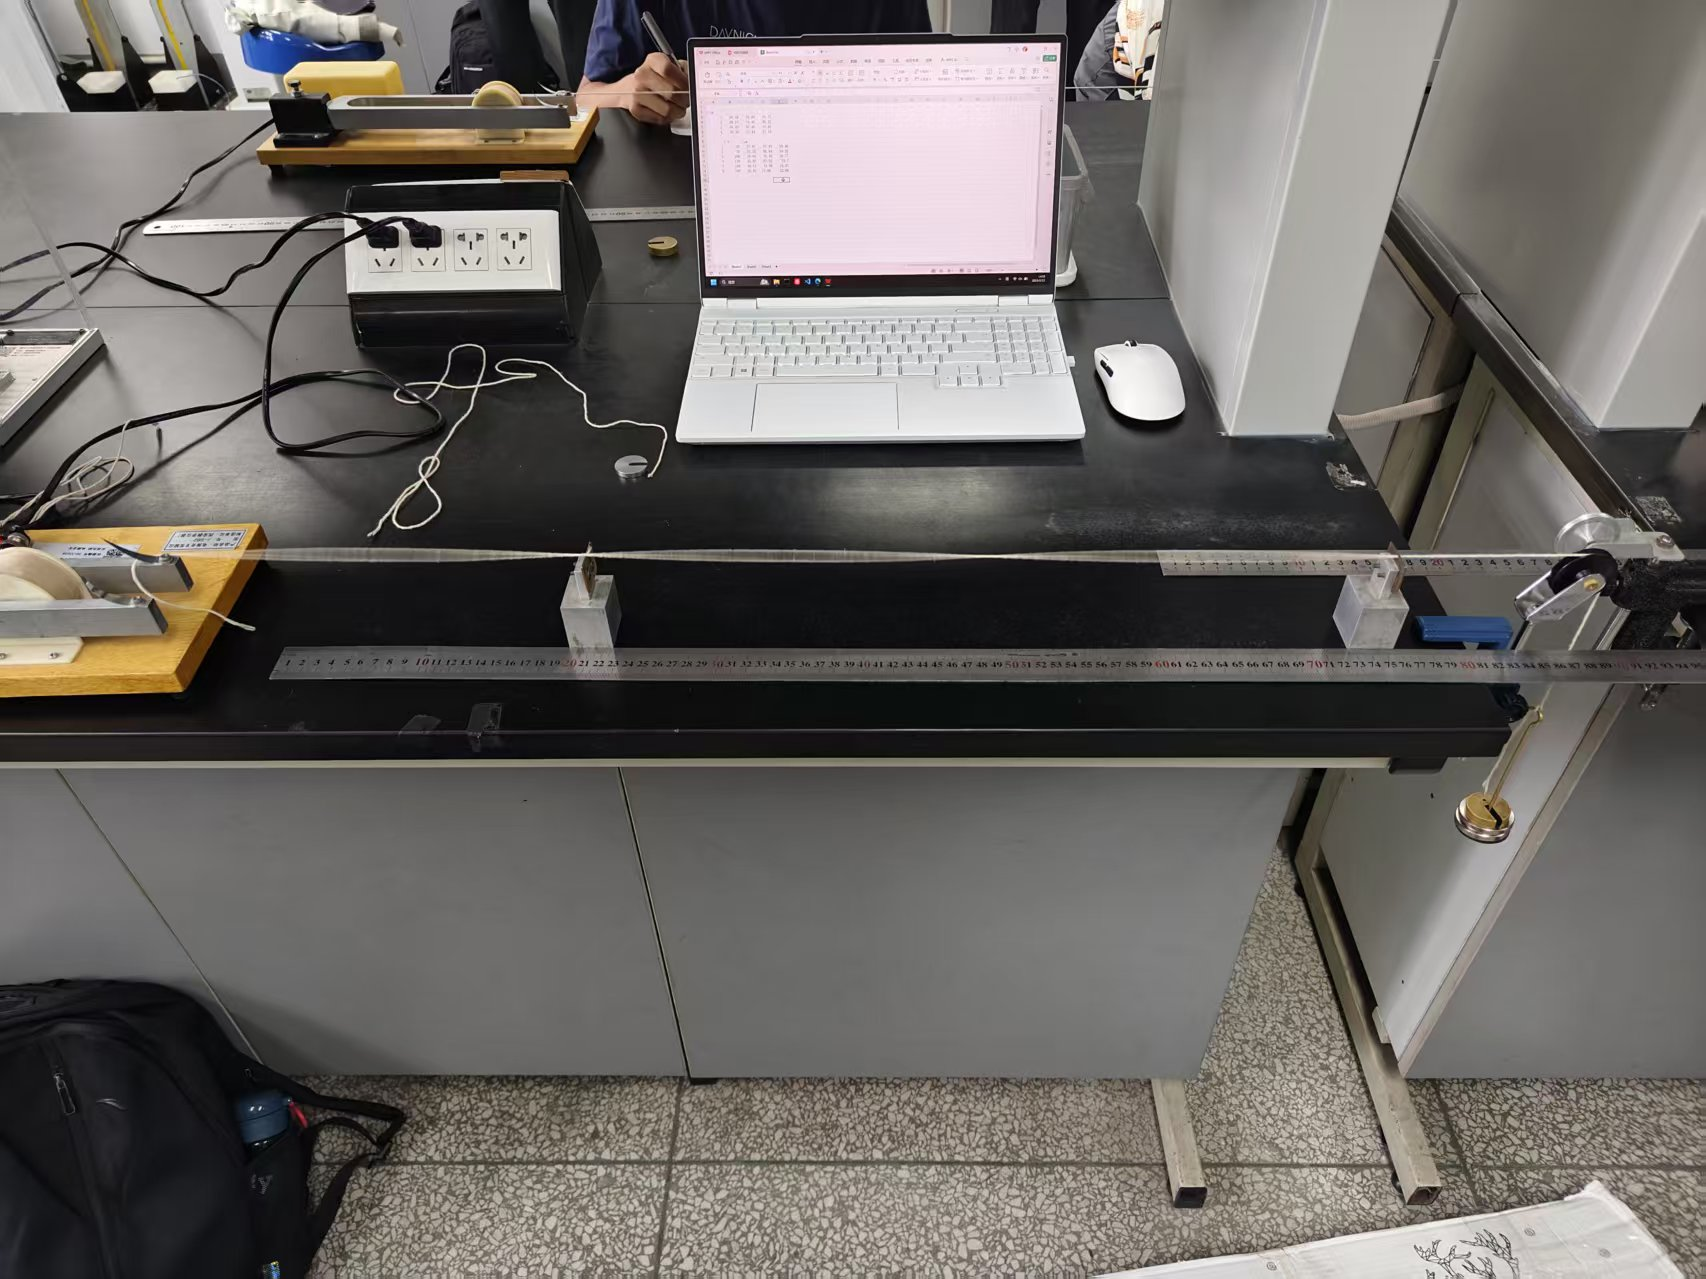
\includegraphics[width=6cm]{3.jpg} % 替换为你的图片路径
    \caption{实验装置}
\end{figure}

\section{实验数据及分析}
\subsection{弦线的线密度$\rho$}
\begin{table}[ht]
    \centering
    \begin{tabular}{ccc}
    \hline \hline
    $L/cm$ & $M/g$  & $\rho/ kg\cdot m^{-1}$   \\
    131  & 0.93 & 0.000709924 \\ \hline \hline
    \end{tabular}
\end{table}

不确定度$u_{\rho}$:
$$
u_M=\frac{0.1g}{\sqrt{3}}=0.057735027\ g \qquad u_L=\frac{0.05cm}{3}=0.016666667\ cm
$$
$$
u_\rho=\rho\sqrt{(\frac{u_M}{M})^2+(\frac{u_L}{L})^2}=4.4\times 10^{-5} \ kg/m
$$

因此,$\rho=7.10\times 10^{-4}\pm 4.4\times 10^{-5}\ kg/m$
\subsection{固定张力$T$,改变$l$}
固定 $T=100\times9.8\times 10^{-3} N$。

\begin{table}[ht]
    \centering
    \begin{tabular}{ccccc}
    \hline \hline
              & 1  &  2    &  3    &   4   \\
    $\lambda/cm$ &39.38 &38.23 &38.44 &38.26  \\ 
    $f/Hz$    & 94.35 &97.19&96.65&97.11\\\hline \hline
    \end{tabular}
\end{table}
计算得到:$\overline{\lambda}=38.5775\ cm$,$\overline{f}=96.32\ Hz$。

1.不确定度$u_\lambda$计算:

$$
\sigma ^2=\sum_{i=1}^{n}\frac{(\lambda_i-\overline{\lambda})^2}{n}=0.2211
$$

$$
S_{\lambda_i}=\sqrt{\sum_{i=1}^{n}\frac{(\lambda_i-\overline{\lambda})^2}{n-1}}=0.5430
$$

$$
S_{\overline{\lambda}}=\frac{S_{\lambda_i}}{\sqrt{n}}=0.2715
$$

$$
u_{a\lambda}=t(0.683,3)S_{\overline{\lambda}}=0.3258\ cm
$$

$$
u_{b\lambda}=\frac{\Delta}{3}=\frac{0.05cm}{3}
$$

$$
u_\lambda=\sqrt{(u_{a\lambda})^2+(u_{b\lambda})^2}=0.33\ cm
$$

2. 不确定度$u_T=\frac{\varepsilon_r}{\sqrt3}=\frac{9.8\times 10^{-3}N}{\sqrt{3}}$

3.不确定度$u_f$计算:
$$
u_f=\overline{f}\sqrt{(\frac{u_\lambda}{\overline{\lambda}})^2+(\frac{u_T}{T})^2+(\frac{u_\rho}{\rho})^2}=3.1\ Hz
$$

综上,$f=\overline{f}\pm u_f=96.3\pm 3.1\ Hz$。

\subsection{固定$l$,改变$T$}

\begin{table}[ht]
    \centering
    \begin{tabular}{ccccccc}
    \hline \hline
              & 1  &  2    &  3    &   4 & 5 &6   \\
    $m/g$&50&70&100&130&160&200\\
    $\sqrt{T}/N^{\frac 12}$ &0.70&0.83&0.99&1.13&1.25&1.40\\
    $\lambda/cm$ &27.97&32.52&38.66&43.82&48.71&53.93\\ 
    $f/Hz$    & 93.93&95.59&96.10&96.67&96.484&97.43\\\hline \hline
    \end{tabular}
\end{table}
计算得到:$\overline{\sqrt{T}}=1.0499\ N^{\frac 12}$,$\overline{\lambda}=40.935\ cm$,$\overline{f}=96.03\ Hz$

1. 使用最小二乘法拟合$\lambda-\sqrt{T}$曲线,并计算$f_{拟合}$:

$$
a_1=\frac{\overline{\lambda\sqrt{T}}-\overline{\lambda}\cdot\overline{\sqrt{T}}}{\overline{T}-\overline{\sqrt{T}}^2}=37.3713\ cm/N^{\frac{1}{2}}
$$
$$
a_0=\overline{\lambda}-a_1\overline{\sqrt{T}}=1.7007\ cm
$$

得到$\lambda=1.7007+37.3713\sqrt{T}$,并作出$\lambda-\sqrt{T}$曲线。

接着计算$f_{拟合}$

$$
f_{拟合}=\frac{1}{a_1\sqrt{\rho}}=100.43\ Hz
$$

\begin{figure}[!ht]
    \centering
    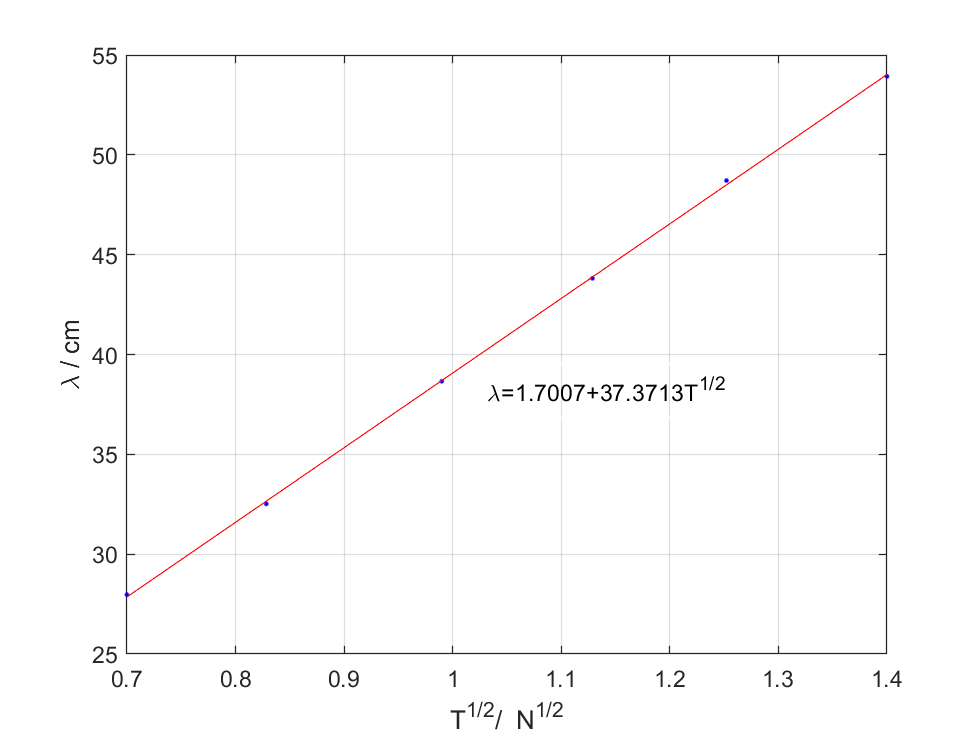
\includegraphics[width=10cm]{4.png}
    \caption{$\lambda-\sqrt{T}拟合曲线$}
\end{figure}

2. 计算最小二乘法的不确定度:
$$
S_{\sqrt{T}\lambda}=\sum_{i=1}^{n}(\sqrt{T_i}-\overline{\sqrt{T}})(\lambda_i-\overline{\lambda})=12.8878
$$
$$
S_{\sqrt{T}\sqrt{T}}=\sum_{i=1}^{n}(\sqrt{T_i}-\overline{\sqrt{T}})^2=0.3449
$$
$$
S_{\lambda\lambda}=\sum_{i=1}^{n}{\lambda_i-\overline{\lambda}}^2=481.7230
$$

不确定度:

$$
u_{\lambda_i}=\sqrt{\sum_{i=1}^{n}\frac{(\lambda_i-a_0-a_1\sqrt{T_i})^2}{n-2}}\ cm
$$
$$
u_{a_1}=\frac{u_{\lambda_i}}{\sqrt{S_{\sqrt{T}\sqrt{T}}}}=0.2534\ cm/N^{\frac{1}{2}}
$$
$$
u_{a_0}=\sqrt{\overline{T}}u_{a_1}=0.2729\ cm
$$
接着转化为$f$的不确定度$u_f$:
$$
f_1=\frac{1}{(a_1+u_{a_1})\sqrt{\rho}}=99.75\ Hz \qquad f_2=\frac{1}{(a_1-u_{a_1})\sqrt{\rho}}=101.11\ Hz
$$
$$
u_{f_1}=f_{拟合}-f_1=0.68\ Hz \qquad u_{f_2}=f_2-f_{拟合}=0.68\ Hz
$$
得到:$u_{f}=0.68\ Hz$

因此,音叉的固定频率$f=f_{拟合}\pm u_f=100.4\pm 0.7\ Hz$。

3.相关系数
$$
r_{\sqrt{T}\lambda}=\frac{S_{\sqrt{T}{\lambda}}}{\sqrt{S_{\sqrt{T}\sqrt{T}}S_{\lambda\lambda}}}=0.9999
$$
可以看出数据的线性相关性较强。

\section{误差分析}
本实验中音叉的固有频率$f_0=100\ Hz$,可以看出实验二比实验一测得的结果更为准确。

其中两个实验都存在的误差有:

1.测量仪器所带来的误差;

2.波节位置的确定存在误差,无法完全精确地确定波节的位置;

3.砝码的微小摆动带来拉力$T$的微小变化;

4.音叉本身振动存在一定的振幅,进而影响弦线的振动。

而实验二通过最小二乘法,计算$\lambda-\sqrt{T}$曲线的斜率从而得到音叉的固有频率$f$,相较于实验一的结果会更加精确,同时不确定度也会更小。

\end{document}